\documentclass{formato/UNIR}

%--- Parámetros de entrada ---%
\titulo{Caracterización de equipos informáticos según su comportamiento en una red empresarial}
\autor{Javier Artiga Garijo}
\director{Luis Miguel Garay Gallastegui}
\fecha{[Fecha de Entrega]}
\ciudad{Logroño}
\universidad{Universidad Internacional de la Rioja (UNIR)}
\escuela{Escuela Superior de Ingeniería y Tecnología}
\master{Máster Universitario en Análisis y Visualización de Datos Masivos}
\tipoTesis{Trabajo Fin de Máster}

\keywords{Plabra clave 1, Palabra clave 2, Palabra Clave N} %Keywords en inglés
\keywordsEs{Plabra clave 1, Palabra clave 2, Palaba Clave N} %Palabras clave en español


%--- Archivo de configuracion global ---%
\makeatletter
    \xdef\autorv{\@author}
    \xdef\titulov{\@title}
    \xdef\masterv{\@master}
    \xdef\fechav{\@date}
    \xdef\universidadv{\@universidad}
    \xdef\escuelav{\@escuela}
    \xdef\tipoTesisv{\@tipoTesis}
    \xdef\directorv{\@director}
    \xdef\ciudadv{\@ciudad}
\makeatother

%Referencias
\usepackage{footmisc}
\usepackage{hyperref}
\hypersetup{
    pdftitle={\titulov},
    pdfauthor={\autorv},
    pdfsubject={\masterv},
    pdfpagemode={UseOutlines},
    bookmarksopen=true,
    bookmarksopenlevel=0,
    hypertexnames=false,
    colorlinks=true,
    pdfborder={0 0 0},
    citecolor=blue,
    linkcolor=blue,
    urlcolor=blue,
    pdfstartview={FitV},
    breaklinks=true
}

%Metadatos
\usepackage{hyperxmp}
\AtBeginDocument{\hypersetup{pdfkeywords={\keywordsESv}}}


%Tablas (líneas horizonales toprule,bottomrule,midrule)
\usepackage{booktabs}

%Estructura del documento
\usepackage[toc,page,title,titletoc]{appendix}
\renewcommand*\appendixpagename{Apéndices}

%Idioma
\usepackage[spanish]{babel}
\addto\captionsspanish{\renewcommand{\tablename}{Tabla}}
\addto\captionsspanish{\renewcommand{\listtablename}{Índice de Tablas}}

%Color azul UNIR
\usepackage[dvipsnames]{xcolor}
\definecolor{azul}{RGB}{81, 131, 187}
\def\azul{\color{azul}}
\def\an{\bfseries\azul}

%Márgenes UNIR
\RequirePackage{geometry}
\geometry{
	paper=a4paper,
	left=3.5cm,
	right=1.5cm,
	top=2.5cm,
	bottom=2.5cm,
	headheight=0.75cm,
	headsep=1.5cm,
	footskip=1.5cm,
	%showframe, % Ver marcos
}

% Cabeceras y pies de página UNIR
\usepackage{lastpage}
\usepackage{fancyhdr}
\pagestyle{fancy}
\patchcmd{\chapter}{\thispagestyle{plain}}{\thispagestyle{fancy}}{}{}

\fancypagestyle{mainmatter}{%
    \fancyhead{}%
    \lhead{{\color{azul}\autorv}}%
    \chead{}%
    \rhead{\masterv}%
    \lfoot{{\color{azul}\titulov}}%
    \cfoot{}%
    \rfoot{\thepage\ of \getpagerefnumber{LastPage}}}

\fancypagestyle{frontmatter}{%
    \fancyhead{}%
    \lhead{{\color{azul}\autorv}}%
    \chead{}%
    \rhead{\masterv}%
    \lfoot{{\color{azul}\titulov}}%
    \cfoot{}%
    \rfoot{\thepage}}

% Necesario para forzar encabezados y pies de página en la primera página de cada
%\usepackage{etoolbox}
\usepackage{setspace} % Espaciado entre líneas
\setstretch{1.5}
\usepackage[autostyle=true]{csquotes} % Referencias en UTF8

% Dependiendo del compilador se utilizan fuentes true type o fuentes convertidas (TFM)
\usepackage{array}
\usepackage{ifluatex,ifxetex}
\ifnum\ifluatex1\else\ifxetex1\else0\fi\fi
    =1 %
        % Fuentes comerciales TTF
    %Fuentes TFM UNIR: Arial, Georgia y Cambria
    \RequirePackage{fontspec}
    
    \setmainfont{Arial}[%
    Path=./formato/fuentes/,
    Extension=.ttf,
    UprightFont =*-Regular,
    BoldFont=*-Bold,
    ItalicFont=*-Italic,
    BoldItalicFont=*-BoldIt]
    
    \newfontfamily{\georgia}{Georgia}%
    [Path = ./formato/fuentes/,
    Extension = .ttf,
    UprightFont = *-Regular,
    BoldFont = *-Bold,
    ItalicFont =*-Italic,
    BoldItalicFont = *-BoldIt]
    
    \newfontfamily{\cambria}{Cambria}%
    [Path = ./formato/fuentes/,
    Extension = .ttf,
    UprightFont = *-Regular,
    BoldFont = *-Bold,
    ItalicFont =*-Italic,
    BoldItalicFont = *-BoldIt]
    
    \newcommand{\cambriamd}{\mdseries \cambria}
    \newcommand{\georgiamd}{\mdseries \georgia}
    \newcommand{\cambriab}{\bfseries \cambria}
    \newcommand{\georgiab}{\bfseries \georgia}

   
  
\else
    \renewcommand{\sfdefault}{arial}
\renewcommand{\familydefault}{\sfdefault}
\newcommand{\arialmd}{\usefont{T1}{arial}{m}{n}}
\newcommand{\arialb}{\usefont{T1}{arial}{b}{n}}
\newcommand{\arialit}{\usefont{T1}{arial}{m}{it}}
\newcommand{\arialbit}{\usefont{T1}{arial}{b}{it}}
\newcommand{\cambriamd}{\usefont{T1}{cambria}{m}{n}}
\newcommand{\cambriab}{\usefont{T1}{cambria}{b}{n}}
\newcommand{\cambriait}{\usefont{T1}{cambria}{m}{it}}
\newcommand{\cambriabit}{\usefont{T1}{cambria}{b}{it}}
\newcommand{\georgiamd}{\usefont{T1}{georgia}{m}{n}}
\newcommand{\georgiab}{\usefont{T1}{georgia}{b}{n}}
\newcommand{\georgiait}{\usefont{T1}{georgia}{m}{it}}
\newcommand{\georgiabit}{\usefont{T1}{georgia}{b}{it}}

\renewcommand{\mdseries}{\arialmd}
\renewcommand{\textmd}[1]{{\arial #1}}
\renewcommand{\bfseries}{\arialb}
\renewcommand{\textbf}[1]{{\arialb #1}}
\renewcommand{\itshape}{\arialit}
\renewcommand{\textit}[1]{{\arialit #1}}
\renewcommand{\normalfont}{\arialmd}
\renewcommand{\textnormal}[1]{{\arialmd #1}}


\fi

%--- Portada ---%
\renewcommand*{\maketitle}{%
    \begin{titlepage}%
        {\flushleft%
            {
\includegraphics[width=8.18cm]{./contenido/img/logo-UNIR.pdf}}\par
        }%
        \vspace{1cm}
        \begin{table}[h!]
        \hyphenpenalty=10000
        \setlength\arrayrulewidth{2pt}
            \begin{tabularx}{14.5cm}{ L{0.074} !{\color{azul}\vline}  L{0.931} }
                & \\
                & \fontsize{14}{14}\selectfont \georgiab \universidadv\\
                & \\
                & \fontsize{18}{18}\selectfont \georgiab \escuelav \\
                & \\
                & \fontsize{14}{14}\selectfont  \georgiab\masterv \\
                & \\ & \\ & \\
                & \fontsize{32}{32}\selectfont \cambriamd \color{azul}   \titulov \\

            \end{tabularx}
        \end{table}
        \vspace{0.5cm}
        {\flushleft \fontsize{11}{11}\selectfont %
            \georgiab \tipoTesisv\par
                \vspace{0.5cm}
                Presentado por: \georgiamd \autorv \par
                \vspace{0.5cm}
                \georgiab Director: \georgiamd \directorv \par
                \vspace{3cm}
                {\color{azul}%
                \georgiab Ciudad: \georgiamd \ciudadv \par
                \georgiab Fecha: \georgiamd \fechav \par}
        }
    \end{titlepage}}

% Símbolos en ecuaciones un poco más grandes
\usepackage{relsize}


%---  Compilacion rapida ---%
% Para ahorrar tiempo de compilación, comentar las secciones que no se quieran compilar
% Carácter % enfrente de la sección.
\includeonly{
  contenido/TFM-00_Abstract,
  contenido/TFM-01_Introduccion,
  contenido/TFM-02_ObjetivosYMetodologia,
  contenido/TFM-03_EstadoDelArte,
  contenido/TFM-04_Desarrollo,
  contenido/TFM-05_Resultados,
  contenido/TFM-06_Conclusiones,
  contenido/TFM-10_Bibliografia,
  contenido/TFM-11_Apendice_1,
%   contenido/TFM-11_Apendice_2 
}

%---------------------------------------------%
%           Inicio del documento
%---------------------------------------------%
\begin{document}
    %--- Páginas iniciales: portada, abstract, índice, lista de figuras y lista de tablas ---%. 
    \frontmatter
    \pagestyle{frontmatter}
      \maketitle          % Portada
      \tableofcontents    % Índice
      \clearpage
      \begin{abstract}[Resumen]
\centering Lorem ipsum dolor sit amet, consectetur adipiscing elit, sed do eiusmod tempor incididunt ut labore et dolore magna aliqua. Ut enim ad minim veniam, quis nostrud exercitation ullamco laboris nisi ut aliquip ex ea commodo consequat. Duis aute irure dolor in reprehenderit in voluptate velit esse cillum dolore eu fugiat nulla pariatur. Excepteur sint occaecat cupidatat non proident, sunt in culpa qui officia deserunt mollit anim id est laborum.\par
\par\vspace{0.25cm}
\centering\textbf{Palabras clave: } \keywordsESv \par
\end{abstract}


\pagebreak
%Ingles
\begin{abstract}
Proin tincidunt enim nec fringilla euismod. Quisque id efficitur sapien. Sed hendrerit, nisl id efficitur elementum, arcu ex efficitur ipsum, sed auctor metus nibh id leo. Maecenas eu sem tortor. Etiam accumsan bibendum ante vitae auctor. Donec eget dolor gravida, tincidunt diam non, ornare orci. Pellentesque ornare blandit eros, sed maximus neque varius non.\par
\par\vspace{0.25cm}
\centering\textbf{Keywords: } \keywordsv \par
\end{abstract}
  %Abtract
      \listoffigures      % Índice de imágenes
      \listoftables       % Índice de tablas
    
    %---    Cuerpo ---% 
    \mainmatter
    \pagestyle{mainmatter}
    %Incluir aquí todos los capítulos (carpeta contenido)
      \chapter{Introducción}\label{chap:introduccion}

El primer capítulo resume de forma esquemática y clara las ideas que componen este trabajo y sobre las que se fundamenta.
En él se presentan elementos como la identificación del problema a tratar, la justificación de su importancia, cómo se vertebra el proyecto y de qué manera contribuye a la resolución de los retos planteados.

\section{Motivación}\label{sec:motivacion}

La monitorización de la red informática en una gran empresa es un problema complejo por muchos factores.
El más inmediato podría ser el alto volumen de conexiones que se producen, superior a varios millones diarios.
Pero se suman otras muchas dificultades a la hora de procesar el tráfico de forma que se obtenga información útil para el analista y, en última instancia, para el cliente final:
la gran variabilidad de comportamientos, la complejidad de sintetizar lo importante sin perder exactitud,
el compromiso entre rapidez en la respuesta y certeza en su fiabilidad, el desconocimiento a priori de cómo se caracteriza un comportamiento anómalo, etc.

Interesa buscar una solución a estos obstáculos porque las empresas quieren garantizar que los recursos de sus redes se gestionan de la manera más óptima posible.
Además, es especialmente importante la seguridad de la red corporativa, esto es, protegerla de acciones no autorizadas u otras amenazas que puedan comprometer su disponibilidad o la integridad de los equipos que la componen.

Equipos de seguridad como puedan ser los firewalls contribuyen de manera decisiva a esta protección, pero su funcionamiento basado en firmas no cubre todos los casos ante una intrusión.
Sin embargo, sí generan una enorme cantidad de datos que, si se tratan adecuadamente, sirven para ampliar el alcance de las técnicas empleadas en materia de seguridad.

Por ello, un sistema que modele el comportamiento normal de una red y detecte anomalías usando métodos estadísticos y de inteligencia artificial permitirá
conocer mejor el contexto de dicha red e identificar comportamientos sospechosos que no se considerarían de otro modo.

\section{Planteamiento del trabajo}\label{sec:objetivos}

Las cuestiones planteadas para guiar esta investigación han sido:
\begin{itemize}
    \item Si podemos clasificar las direcciones IP de una gran red empresarial en categorías relevantes según su comportamiento de red
    \item Cuáles serían esas categorías
    \item Si sereremos capaces de identificar comportamientos sospechosos en base a esta clasificación
\end{itemize}

A través de estas cuestiones se inicia el estudio del problema, para cuya solución se propone obtener un modelo clasificador que distinga patrones de comportamiento normales y desviaciones respecto de la actividad normal.
Este clasificador se realizará mediante una técnica de aprendizaje automático no supervisado como es el \emph{clustering} (técnica que lleva a cabo una agrupación en categorías de manera natural, buscando características en común sin haber definido las clases previamente).

El objetivo principal es localizar en la red interna orígenes de tráfico catalogable como extraño, lo que puede indicar un equipo infectado o mal configurado.
La determinación de qué se sale de lo habitual dependerá de las particularidades de la red, algo difícil de concretar a priori y más aún de generalizar,
razón por la cual el \emph{clustering} (como etapa final tras un análisis y preprocesado de los datos adaptado al caso) se ha considerado una técnica idónea en esta tarea.

\section{Estructura del documento}\label{sec:estructura}

Una vez expuesto en este capítulo \ref{chap:introduccion} el problema que se va a abordar durante este trabajo y cómo se enfoca su estudio,
se dedica el capítulo \ref{chap:objetivos} a definir los objetivos, tanto generales como específicos, hacia los que se dirigirá el proyecto.
También se incluye en él la metodología seguida.
Esta explica qué pasos se dan en la aplicación del \emph{clustering} a este caso, el por qué de cada paso, qué instrumentos se van a utilizar, cómo se analizan los resultados, etc.

El capítulo \ref{chap:estadodelarte} dota de contexto científico a este trabajo: se revisa el estado del arte.
Mediante la relación de diversos artículos y publicaciones académicas sobre aprendizaje automático aplicada a la clasificación de tráfico,
en esta parte de la memoria se sintetizan los conceptos fundamentales y los hallazgos más relevantes para este campo.
Se diferencian distintos enfoques en la detección de anomalías, valorando los aspectos positivos y las desventajas de cada uno.
Para cerrar, se justifican las decisiones tomadas con las que, sobre el conocimiento disponible en torno al tema, sentar las bases del desarrollo de este piloto.

En el capítulo \ref{chap:desarrollo} se entra en los detalles del desarrollo.
Paso a paso, se profundiza en todos los puntos que se han recorrido hasta alcanzar unos resultados satisfactorios.
Esto incluye: presentación del escenario, trabajo con estándares y \emph{scripts} para extraer de los datos en bruto la información útil para el propósito actual,
análisis estadístico de las variables, selección de estas y parametrización del algoritmo K-Means para obtener una clasificación.
Todo ello se ha ido conseguiendo y mejorando de forma incremental, volviendo atrás e incorporando avances.
En el capítulo se presenta ordenadamente, siguiendo la línea a través de la cual los datos se transforman por etapas hasta tener finalmente la clasificación de los equipos.

Es entonces cuando se pasa al capítulo \ref{chap:resultados}: resultados.
Ahí se describe más ampliamente y se analiza la salida del algoritmo, evaluando cómo se han compuesto los \emph{clusters} y qué indicadores reflejan la calidad del resultado.
Se interpreta el valor del mismo y qué significa este resultado de cara a los objetivos marcados.

En último lugar, el capítulo \ref{chap:conclusiones} recoge las conclusiones derivadas del trabajo realizado.
Se comentan también las líneas futuras que este piloto podría seguir para evolucionar.

      \chapter{Objetivos y metodología}\label{chap:objetivos}

Se procede a explicar en este capítulo los objetivos concretos y la metodología de trabajo que van a marcar cómo se materializará la contribución que se va a realizar.

\section{Objetivo general}\label{sec:objgeneral}
El objetivo general del presente trabajo es extender la capacidad de monitorización que se tiene sobre una red empresarial.
Se enfocará para ello en la detección de anomalías, haciendo uso de técnicas basadas en los equipos que la componen (a diferencia de las basadas en flujos de tráfico).
De este modo, se desarrollará un sistema que categorice mediante \emph{clustering} los equipos informáticos finales (es decir, todos menos la infraestructura de la red)
y que pueda revelar cuándo la actividad de un equipo se desvía de su comportamiento habitual.

Con ello se espera seguir mejorando las prestaciones ofrecidas, especialmente en seguridad, pero también ayudará en la identificación de problemas de configuración, cambios de tendencia en la red y en definitiva cualquier evento inesperado que pudiera repercutir negativamente en la operativa normal de la empresa monitorizada.

\section{Objetivos específicos}\label{sec:objespecificos}
La consecución de dicho objetivo general vendrá pautada por las siguientes metas más específicas, que se abordarán en este orden:

\begin{itemize}

\item Determinar qué características son las más relevantes a la hora de \emph{clusterizar} la red y extraerlas en tiempo real.

\item Establecer unas categorías básicas mediante clasificación no supervisada, que sean verificables con la documentación que se tiene de la red.

\item Comprobar que el sistema detecta anomalías.

\item Refinar el algoritmo de \emph{clustering} empleado, buscando categorías más específicas que no se estuvieran teniendo en cuenta antes.

\item Alcanzar un modo de funcionamiento en tiempo real, en coordinación con los demás mecanismos de monitorización presentes y asegurando una precisión razonable.

\end{itemize}

\section{Metodología de trabajo}\label{sec:metodologiatrabajo}

Con los anteriores objetivos específicos marcados, se hace necesario establecer un marco de trabajo para llevarlos a cabo.
En esta sección se estructurará una metodología de trabajo en base a cuatro fases, que tienen como fin último alcanzar el objetivo general.
Sus enunciados vendrán acompañados de una descripción, explicando con un poco más de detalle cómo se planea ejecutar cada etapa.

\begin{itemize}

    \item Selección de las características más relevantes para la clasificación

A partir de la heterogénea colección de logs de varios firewalls de la que se dispone, se identificarán los datos que puedan ser interesantes para el \emph{clustering}.
Se tendrán en cuenta distintos aspectos que respondan a las actividades que realiza un equipo informático en una red empresarial, como por ejemplo la cantidad de conexiones, sus duraciones, horarios de actividad, interacción con ciertos servidores, etc.
A continuación, se analizarán estas características a través de técnicas estadísticas, gracias a las cuales se adquirirá un entendimiento preliminar de la importancia que cada una supone para la posterior clasificación de instancias.
Es posible que se logre la reducción de su dimensionalidad, la eliminación de alguna característica redundante o en definitiva alguna simplificación que haga el \emph{clustering} más sencillo de ejecutar.

    \item Obtención de categorías mediante \emph{clustering}

Se pasará entonces a aplicar por primera vez algunos métodos de \emph{clustering} sobre estos datos.
Lo que se pretende es categorizar los equipos en su comportamiento ``normal'', de forma que se tengan clasificados en varios tipos según su actividad.
Inicialmente se elegirá un algoritmo simple y ampliamente conocido como es K-Means, con variaciones sobre él.
Se experimentará con diferentes valores para sus parámetros, ya que así podrán compararse resultados.
De cara a determinar la efectividad de los algoritmos, se considerarán medidas objetivas que representen su rendimiento.
Los métodos típicos para ello valoran características intrínsecas o derivadas como su complejidad, estabilidad y tiempo de computación, así como la suma de cuadrados de las desviaciones.
Además, se emplearán los indicadores comunes con los que se suele definir la bondad de una técnica de clasificación en aprendizaje automático.

    \item Detección de anomalías con análisis del \emph{clustering}

Una vez se cuente con una clasificación satisfactoria, se procederá a la siguiente fase, en la cual se aspira a detectar anomalías en los datos.
En caso de contar con instancias que se hayan identificado como anomalías mediante otros métodos, se usarán para probar la capacidad de detección del sistema.
Dado que también se desea detectar otras clases de anomalías más genéricas (no solo relacionadas con seguridad), se incluirán casos como cambios de configuración o de equipos que hayan cambiado de rol en la red.

    \item Evaluación en escenario real

Finalmente, se desplegará el sistema desarrollado en un entorno de producción.
Se ofrecerá una representación visual adecuada que permita al analista aprovechar el valor que el sistema aportará a la hora de revisar casos alertados.
Además, se automatizará la extracción de características y se prepararán el resto de componentes del sistema para que funcione lo más cercano a tiempo real posible.

\end{itemize}

\section{Metodología del desarrollo}\label{sec:metodologiadesarrollo}

Tras haber completado las fases del desarrollo requeridas para poner en funcionamiento este piloto y haber analizado y probado lo que mejor funcionaba en cada una,
se ha plasmado la metodología seguida en esta serie de pasos, que ofrecen una visión global del desarrollo que se ampliará en el capítulo \ref{chap:desarrollo}:

\begin{itemize}

\item A partir de logs en bruto de firewall, extracción de los vectores de características de las sesiones.

\item Preprocesado antes del \emph{clustering}:

    \begin{itemize}

        \item Muestreo (necesario para el desarrollo, pero prescindible cuando se lleve a producción).

        \item Transformación de los datos individuales en características para la entrada del \emph{clustering},
            formada básicamente, por un lado, por la agrupación diaria y por IP origen, y por otro, por el cálculo de las métricas con las que se ha decidido trabajar.

        \item Estandarización de estos datos.

    \end{itemize}

\item Aplicación de KMeans con $k=5$

\item Análisis:

    \begin{itemize}

        \item Revisión manual en el entorno de la empresa de las IP clasificadas como anomalías.

        \item Evaluación de la estabilidad del resto de \emph{clusters} normales, para vigilar si hay cambios de tendencia.

    \end{itemize}

\end{itemize}

El siguiente esquema de la figura \ref{fig:esquema} resume todo el procesado:

\begin{figure}[h]
    \centering
    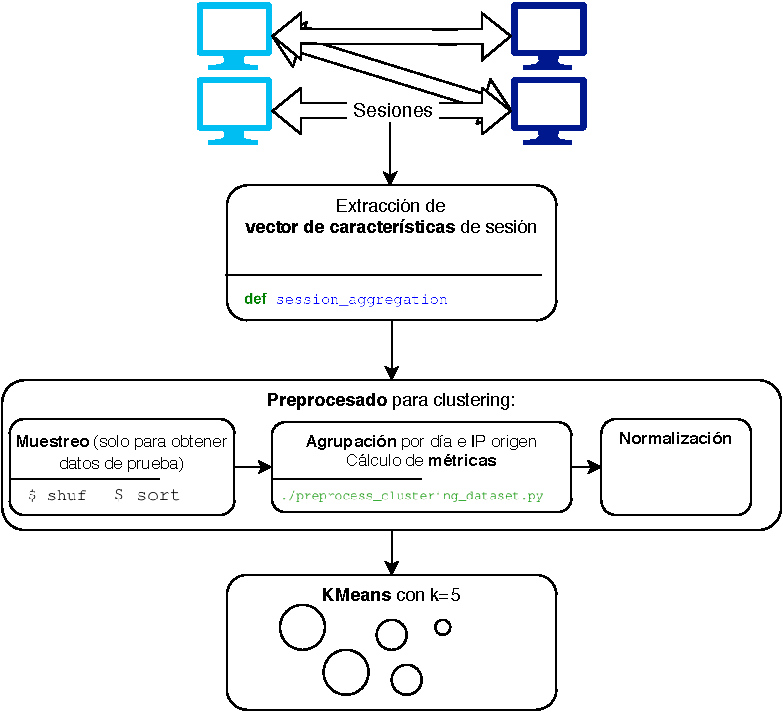
\includegraphics{contenido/fig/esquema.pdf}
    \caption{Diagrama de la metodología seguida en el procesado}
    \label{fig:esquema}
\end{figure}

      \chapter{Estado del Arte}\label{chap:estadodelarte}
\textbf{Contexto y estado del arte}

%Párrafo introductorio del capítulo
[Párrafo introductorio del capítulo. Lorem ipsum dolor sit amet, consectetur adipisicing elit. Natus impedit sint cumque, omnis assumenda, molestias corporis repellat, reprehenderit, ullam labore aliquam. Velit ut, ab amet a recusandae, eaque similique alias!]

\section{Aprendizaje automático en la clasificación de tráfico}\label{sec:aprendizajeautomaticoenclasiftrafico}

El aprendizaje automático puede resumirse como una colección de técnicas de gran potencial para la minería de datos y el descubrimiento de conocimiento \cite{NA08}.
En concreto, a la hora de extraer este conocimiento, estas técnicas son especialmente eficaces buscando y describiendo patrones estructurales útiles en los datos.
Además, la ventaja intrínseca de esta disciplina frente a la exploración que pueda efectuar un especialista es que, al poder definirse algorítmicamente el procedimiento para su aplicación, se hace posible implementar sistemas automatizados sobre equipos informáticos.

Un sistema de \emph{machine learning} aprende automáticamente de la experiencia y perfecciona su base de conocimiento, entendiendo ``aprender'' como la acción de mejorar su rendimiento en el desempeño de una tarea determinada \cite{Simon_1983}.
Esta mejora debe ser cuantificable objetivamente en base a lo que se denomina como medida de rendimiento.
El sistema (como cualquier otro agente computacional en la rama de la inteligencia artificial) recibirá estímulos externos (en este caso, conjuntos de datos) y,
en base a ellos y al conocimiento que recogen el algoritmo y los resultados de sus ejecuciones previas, producirá una salida que maximizará la medida de rendimiento establecida.

En terminología de \emph{machine learning}, el conjunto de datos que se toma como entrada se compone de instancias.
Una \emph{instancia} simboliza a un individuo específico de la población sobre la que se trabaja.
Cada instancia se representa por sus valores en una serie de \emph{características} o atributos, que no son más que medidas sobre aspectos de interés para el escenario en cuestión.
Un conjunto de instancias con ciertas características comunes pertenece a una \emph{clase} o concepto.
De este modo, se aprende un concepto cuando, dada una instancia, se logra identificar correctamente con qué clase se corresponde.
Este aprendizaje implica también que se es capaz tanto de generalizar la aplicación del nombre de la clase a todos los miembros de la misma como de discriminar a los miembros que pertenecen a otra clase.

Atendiendo a la naturaleza de las clases resultantes, los tipos de aprendizaje se dividen en aprendizaje supervisado y no supervisado.
El primer tipo es capaz de clasificar nuevas instancias en clases predefinidas.
Por el contrario, el segundo clasifica las instancias en clases no definidas con anterioridad.
La técnica de aprendizaje no supervisado principal es el \emph{clustering} o agrupamiento, que se explicará con detalle más adelante.

En los últimos tiempos, el aprendizaje automático se ha venido usando cada vez más en la clasificación de tráfico IP \cite{Dainotti_2012}.
Las técnicas de clasificación de tráfico siguen mejorando en acierto y eficiencia, pero
la proliferación constante de aplicaciones en Internet con comportamientos muy variados, sumado a
los incentivos que tienen ciertos agentes para enmascarar algunas aplicaciones y así evitar el filtrado o bloqueo en firewalls,
son algunas de las razones por las que la clasificación de tráfico permanece como uno de los muchos problemas abiertos de Internet.
Han quedado obsoletos métodos clásicos como la identificación de aplicaciones en base a sus puertos conocidos (aquellos registrados por la IANA), que resulta muy simple y rápida pero también poco fiable.
En el otro extremo, las técnicas de ``Deep Packet Inspection'', que analizan en profundidad el funcionamiento de las aplicaciones desde la perspectiva de su uso de los protocolos o
buscan datos específicos en paquetes IP para inferir a qué aplicación pertenecen, suponen una alta carga computacional y habitualmente requieren hardware específico.
Además, el buen funcionamiento de un clasificador DPI está supeditado a dos condiciones: que pueda inspeccionar el contenido de los paquetes IP y que sepa cómo interpretar la sintaxis de cada aplicación.
La primera condición queda comprometida por la estandarización de las conexiones cifradas,
mientras que la viabilidad de la segunda se vería restringida por la complejidad de contar con un repositorio completo y constantemente actualizado del formato de los paquetes que puede generar cada aplicación.
Ante estas técnicas también se presentan dificultades legales y relacionadas con la privacidad.

Si se trata de clasificadores de tráfico, lo más común es encontrar planteamientos basados en flujos de tráfico.
En ocasiones, la granularidad de la clasificación se afina hasta el uso de flujos bidireccionales (asumiendo que se tiene visibilidad de ambas direcciones), pero operar a este nivel entraña una complejidad bastante mayor.
Un flujo se suele definir como una tupla de 5 elementos: protocolo de transporte (frecuentemente, TCP o UDP), direcciones IP de origen y destino, y puertos de origen y destino.
Con este concepto como \emph{objeto} fundamental, tradicionalmente se han buscado patrones estadísticos en los atributos de los flujos que son observables desde una perspectiva externa (es decir, sin considerar el contenido o \emph{payload} de los paquetes).
Ejemplos de estos atributos serían: tamaño de paquetes, tiempo entre llegadas, número de paquetes en cada dirección, duración total... resumido cada uno con el estadístico muestral que se considere adecuado.
Con la popularización del aprendizaje automático, se ha podido llevar la búsqueda de patrones entre dichos atributos a nuevos grados de profundidad.

Se trabaja también con otras variantes en cuanto a cómo agrupar los paquetes que se hayan intercambiado dos máquinas.
Entre ellas, podrían destacarse las conexiones TCP o los servicios, definidos estos como el tráfico generado entre una pareja de IPs-puertos.
En cualquiera de los casos anteriores, se pone el foco sobre flujos individuales, para después clasificarlos bajo categorías que comparten características.
Este tipo de planteamientos no tienen tan en cuenta el conjunto de acciones que lleva a cabo un mismo equipo.
Así, se corre el riesgo de perder información útil de cara a entender de forma completa qué es realmente lo que están haciendo los equipos de la red.

Por otro lado, se encuentran los clasificadores de tráfico basados en el comportamiento del host.
Sirva de referente el trabajo de \cite{KPF05}, donde se propuso un novedoso método que identificaba patrones en el comportamiento de los hosts a la altura de la capa de transporte.
Se trataba de una aproximación multinivel que descartaba incluir datos sobre el payload, los puertos bien conocidos (aspectos que conllevan las problemáticas anteriormente comentadas) o cualquier otra información separada de la que ofrecían los colectores de flujos.
Consistía por tanto en un clasificador ``a ciegas'' (\emph{``BLINd Classification'', abreviado como ``BLINC''}) que analizaba cada hosts desde tres perspectivas: social, funcional y aplicativa.
La perspectiva social capturaba las interacciones del host con otros hosts, en términos de cuántos hosts se conectaban con qué hosts.
La funcional los separaba según actuaran como proveedores de un servicio, consumidores o ambos.
Se tenían en cuenta, por tanto, los roles del modelo cliente-servidor.
Por último, en la perspectiva aplicativa se utilizaba la información de la capa de transporte con la intención de distinguir la aplicación en cuestión.

Mediante la premisa de no tratar cada flujo como una entidad distinta, se conseguiría acumular la información necesaria para reconocer el verdadero comportamiento de cada host.
Además de cumplir con la identificación de aplicaciones específicas, este método sería resistente a circunstancias de la red como congestión o cambios de rutas.
Esto es así porque, a diferencia de otros métodos (véanse los mencionados sobre flujos), una aproximación centrada en el comportamiento de los hosts suele ser insensible a las variaciones que puedan presentar parámetros como los tiempos de llegada entre paquetes.
En cuanto a resultados, los enfoques de aprendizaje automático basados en patrones de comunicación de los hosts alcanzan resultados comparables a los de técnicas de DPI, siendo notablemente más asequibles y menos invasivos con la privacidad.

Es por todo lo anterior que en los sistemas de detección de intrusiones, que se van a desarrollar en la siguiente sección, priman los enfoques sobre el host en vez de sobre el flujo.

\section{Detección de anomalías sobre actividad de red}\label{detectanomsobreactividadred}

En la gestión y monitorización de una red empresarial cobra especial relevancia la seguridad.
En este ámbito, la seguridad informática se centra en proteger la red corporativa de ataques que puedan comprometer su disponibilidad o la integridad de los equipos que la componen, así como
bloquear acciones no autorizadas y evitar el uso indebido de los recursos que quedan expuestos al exterior.

Las organizaciones toman numerosas medidas de seguridad frente a estas amenazas, tanto \emph{software} como \emph{hardware}.
Dos ejemplos claros serían los antivirus y los firewalls, que podríamos englobar dentro de las aproximaciones a la seguridad basadas en firmas \cite{Alconzo_2019}.
Sin embargo, estos métodos dependen de que el fabricante del producto de seguridad haya detectado el ataque previamente, haya generado una firma que lo identifique y haya distribuido la misma hasta el cliente final.
Es decir, solo pueden ofrecer protección ante ataques conocidos y requieren que todos los pasos anteriores se hayan completado.

En contraposición, existen los sistemas de seguridad basados en detección de anomalías.
Este tipo de métodos asumen que el impacto de un ataque modificará el comportamiento de la red, así que construyen un modelo que represente el comportamiento normal de la red, especificado por ciertas métricas.
A continuación, monitorizan el tráfico y fijan alarmas que se dispararán cuando el valor recogido en alguna de esas métricas de referencia se desvíe del rango considerado normal \cite{Boutaba_2018}.

Habitualmente, este tipo de defensas basadas en detección de anomalías son complementarias a las basadas en firmas.
Se sitúan en una segunda línea con el objetivo de detectar a tiempo síntomas tempranos de ciberataques, para así poder actuar antes de que causen daños.
Ambos enfoques pueden encontrarse integrados en soluciones conocidas como IDS/IPS (\emph{Intrusion Detecion/Prevention System}).

Hablando en términos generales, pueden distinguirse tres fases básicas que cumplen todos los NIDS (\emph{Network} IDS) basados en anomalías \cite{GarciaTeodoro_2009}:
\begin{itemize}
    \item \emph{Parametrización}: las instancias del sistema objetivo se representan de forma adecuada para su tratamiento.
    \item \emph{Entrenamiento}: se caracteriza el comportamiento normal del sistema, mediante un modelo que puede construirse con técnicas basadas en alguna de las categorías descritas después.
    \item \emph{Detección}: se compara el modelo con el tráfico disponible, de forma que se dispara una alarma si una instancia se desvía.
\end{itemize}

Según cómo se modele el comportamiento normal del sistema \cite{Lazaveric_2005}, las técnicas pueden categorizarse en: basadas en estadística, en conocimiento o en aprendizaje automático.
Las primeras no requieren un conocimiento previo sobre la actividad normal del sistema, pero la presunción que asumen de cuasi-estacionalidad es poco realista.
Las segundas son robustas, pero el mantenimiento de datos de calidad resulta difícil y costoso.
En cuanto a las técnicas basadas en aprendizaje automático, son flexibles y adaptables.
También pueden capturar interdependencias entre las variables que no son fáciles de encontrar de otra forma.
No obstante, estas técnicas tienen una dependencia importante de lo que se acepte como comportamiento normal.

Para este trabajo, se ha elegido desarrollar un sistema de detección de anomalías basado en una técnica de aprendizaje automático como es el \emph{clustering}.

En \cite{Alconzo_2019} se resaltan acertadamente las bondades y debilidades de los métodos de detección de anomalías, al decir que ``son atractivos porque permiten la pronta detección de amenazas desconocidas (por ejemplo, zero-days).
Estos métodos, sin embargo, puede que no detecten ataques sigilosos, insuficientemente amplios para perturbar la red.
A veces también adolecen de un alto número de falsos positivos.''

Continúa señalando cómo beneficia el aprendizaje automático a este tipo de sistemas: ``el \emph{machine learning} ha recibido una significativa atención en la detección de anomalías, debido a
la autonomía y robustez que ofrece en el aprendizaje y también a la hora de adaptar el perfil de la normalidad según va cambiando.
Con \emph{machine learning}, el sistema puede aprender patrones de comportamientos normales dentro de entornos, aplicaciones, grupos de usuarios y a lo largo del tiempo.
Además, ofrece la capacidad de encontrar correlaciones complejas en los datos que no pueden deducirse de la mera observación''.

Se concluye por tanto que la obtención de una representación completa de la normalidad, requisito no trivial en estos sistemas basados en detección de anomalías, puede tomarse como un problema de clasificación en instancias normales y no normales.
Dicho problema puede abordarse mediante la técnica de aprendizaje no supervisado descrita a continuación.

\section{Clustering}\label{clustering}

El clustering se define en \cite{NA08} como la agrupación de instancias que tienen características \emph{cercanas} en forma de clusters, sin aplicar ninguna orientación previa.
Esta técnica de aprendizaje automático no supervisado asocia a las instancias con propiedades similares bajo el mismo grupo,
determinando dicha similaridad en un modelo que posibilite la medición de distancias específicas, como pueda ser el espacio euclídeo.
Los grupos pueden ser exclusivos, si cada instancia pertenece a un único grupo; solapados, si una instancia puede pertenecer a varios grupos; o probabilísticos, si la pertenencia de una instancia a un grupo se expresa mediante una cierta probabilidad.

El primer uso de clustering para detección de intrusiones se vio en \cite{Portnoy_2000}.
La hipótesis en base a la cual los autores aplicaron clustering para esta tarea es que las conexiones entre datos normales crearán clusters más grandes y más densos.
Si se lleva el análisis un paso más allá, para incrementar la precisión de la técnica, además de las consideraciones anteriores debe tenerse en cuenta la distancia entre clusters, como se demuestra en \cite{JSW+06}.

Los tipos de algoritmos de clustering usados en clasificación de tráfico son variados.
En \cite{MHL+04} se aplica por primera vez un algoritmo de clustering probabilístico como es \emph{Expectation Maximization} sobre flujos de tráfico.
Considerando varias estadísticas sobre longitud de paquetes, tiempos entre llegadas, cantidad de bytes, duración de la conexión y número de permutaciones de modo ``transaccional'' a modo ``por lotes'' (y viceversa),
se consigue una clasificación con baja granularidad.
Otros estudios valoran más medidas estadísticas
[Más algoritmos de clustering en clasif de tráfico:
- AutoClass (Zander et al.):
    - features: packet length stats (mean, variance in forward and backward directions), inter-arrival stats (mean, var. in f-b dirs), flow size (bytes), flow duration. Calculated on full flows
    - classif level: (muy granular) 8 aplicaciones estudiadas
- K-Means (Bernaille et al.):
    - features: Packet lengths of the first few packets of bi-directional traffic flows
    - features: (muy granular) 10 aplicaciones estudiadas
]

[Algoritmos de clustering en detección de anomalías:
\cite{Syarif_2012} % ((Unsupervised clustering approach for network anomaly detection))
\cite{Leung_2005} % ((Unsupervised Anomaly Detection in Network Intrusion Detection Using Clusters))
\cite{Kim_2018} % ((Multivariate network traffic analysis using clustered patterns))
]

[Network-IDS basados en anomalías. Medidas de validación de clusters:
\cite{Bhuyan_2014} % Anomaly-based network intrusion detection: Techniques, systems and challenges
]

[Conclusiones sobre los trabajos previos]

      \chapter{Desarrollo}\label{chap:desarrollo}
\textbf{Desarrollo específico de la contribución}

%Párrafo introductorio del capítulo
[Párrafo introductorio del capítulo. Lorem ipsum dolor sit amet, consectetur adipisicing elit. Natus impedit sint cumque, omnis assumenda, molestias corporis repellat, reprehenderit, ullam labore aliquam. Velit ut, ab amet a recusandae, eaque similique alias!]

\section{Presentación del entorno}\label{sec:presentaciondelentorno}

En el escenario del proyecto (la red de un banco que es cliente de la empresa),

\section{Extracción y filtrado}\label{sec:extraccionyfiltrado}

El punto de interés para la captura se concentra por tanto en dos equipos por los que pasa el grueso del tráfico total: un Firewall Fortinet y un IPS PaloAlto.
Como es habitual, estos equipos reportan todas sus acciones a través de logs, con varios niveles de granularidad e importancia.
Incluyen también multitud de información aportada por los propios sistemas que enriquecen el valor de cada evento.
Esto es razón para preferir los logs de firewall como fuente de información frente a una captura de tráfico en crudo, ya que
lo que procesan los firewalls casi siempre es más relevante que el tráfico completo pero sin procesar.
Además, el volumen de una captura de tráfico de estas características sería notablemente mayor y más difícil de manejar.

Aunque el fin para el que sirven ambos equipos (análisis y protección frente a amenazas informáticas) sea similar, la estructura usada por cada uno en los logs que produce es completamente distinta.
Los logs de Fortinet siguen un formato clave-valor con ciertas particularidades, mientras que los de PaloAlto tienen una serie de campos fijos que están delimitados por comas. A modo de ejemplo, las líneas adjuntadas a continuación corresponden a un evento del firewall Fortinet y otro del IPS PaloAlto, respectivamente (cada línea es un evento):

\begingroup
\makeatletter
\@totalleftmargin=-1cm
\begin{verbatim}

1585572524|1585572524|2020-03-30T06:48:44.202297-06:00|10.2.0.11|6|local7|
date=2020-03-30 time=06:48:44 devname="FW1_INTERNETCORP" devid="FG1809999"
logid="1059028704" type="utm" subtype="app-ctrl" eventtype="app-ctrl-all"
level="information" vd="root" eventtime=1585572524 appid=41470 user="NOM"
group="GrupoOffice365" authserver="SV1" srcip=172.2.9.6 dstip=23.203.51.72
srcport=54697 dstport=443 srcintf="p18" srcintfrole="undef" dstintf="p20"
dstintfrole="wan" proto=6 service="HTTPS" direction="outgoing" policyid=124
sessionid=325186437 applist="AC_CORREO" appcat="Collab" app="Microsoft.CDN"
action="pass" hostname="img-prod-cms-rt-microsoft-com.akamaized.net"
incidentserialno=1513678724 url="/" msg="Collaboration: Microsoft.CDN,"
apprisk="elevated" scertcname="a248.e.akamai.net"

1585659863|1585659863|2020-03-31T07:04:23.027791-06:00|10.2.0.73|6|local0|
1,2020/03/31 07:04:23,001801037558,TRAFFIC,end,2049,2020/03/31 07:04:03,
10.138.4.7,186.151.236.155,0.0.0.0,0.0.0.0,OUTBOUND,,,incomplete,vsys1,
trust,untrust,ethernet1/10,ethernet1/9,Log-Panorama,2020/03/31 07:04:03,
41602,1,55074,80,0,0,0x19,tcp,allow,132,132,0,2,2020/03/31 07:03:55,3,any,
0,1307298109,0x80000,10.0.0.0-10.255.255.255,America,0,2,0,aged-out,13,0,0,
0,,PA-3020-Z9,from-policy,,,0,,0,,N/A,0,0,0,0

\end{verbatim}
\endgroup

Volumen de estos logs

Otro hecho reseñable que afecta al formato es que se emplea \emph{syslog}\footnote{\url{https://tools.ietf.org/html/rfc5424}} como protocolo para trasladar los datos desde cada equipo hasta la sonda, de forma que se cuenta con ciertos campos adicionales a los enviados por los equipos.
Para el tema que nos ocupa, el único campo que se extrae de esta cabecera es la marca de tiempo en la que ha llegado cada evento, conocida en el vocabulario informático como \emph{timestamp}.
En cualquier caso, esta sección adicional dentro de los logs tiene también su propio formato, por lo cual también se deberá tratar de forma específica.
En nuestra configuración (que aplica a la herramienta \emph{rsyslog}\footnote{\url{https://www.rsyslog.com/}}), la siguiente directiva establece cómo se vuelcan a fichero estos campos de syslog:

\begin{verbatim}
template(name="FORMATO_LOGS" type="string"
string="%timereported:::date-unixtimestamp%|
    %timegenerated:::date-unixtimestamp%
    |%timegenerated:::date-rfc3339%|%fromhost-ip%
    |%syslogseverity%|%syslogfacility-text%| %syslogtag%%msg%\n")
\end{verbatim}

Así que, en los \emph{scripts} que procesan los ficheros donde se han volcado los datos traídos mediante \emph{syslog}, la fecha de cada evento se obtiene a partir de este primer campo ``timereported:::date-unixtimestamp''.
Esta primera parte del procesado, expresada en Python, se hace de la siguiente manera:

\begin{minted}{python}
for syslogline in sys.stdin:

    try:

        splitted_syslogline = syslogline.rstrip().split("|") # .rstrip() removes last "\n" character

        tstamp_line = int(splitted_syslogline[0])
\end{minted}

Adelgazado de logs.

Agregación de sesiones.

\section{Preprocesado para el clustering}\label{sec:preprocesado}

\section{Exploración de datos}\label{sec:exploraciondedatos}

\section{Selección de características}\label{sec:selecciondecaracteristicas}

      \chapter{Resultados}\label{chap:resultados}

El penúltimo capítulo se dedica a analizar los resultados obtenidos en la iteración final de las adelantadas en el capítulo \ref{chap:desarrollo} ``Desarrollo''.
Se ahonda en aspectos como las proporciones y composición de los \emph{clusters}, sus centroides, métricas de bondad y en definitiva se explica qué significan estos resultados para este trabajo.
Sobre todo, se evalúa cómo contribuye este trabajo al objetivo establecido inicialmente.

\section{Composición de los clusters}\label{sec:composicionclusters}

Como se adelantaba en la página anterior, más del 80 \% de los equipos de la red se clasifican como comportamientos totalmente normales (subdivididos en dos categorías: normal con muchas conexiones distintas y normal con pocas conexiones).
Algo menos del 10 \% se agrupan en una tercera categoría porque el tráfico de los equipos que la forman es mayoritariamente UDP (lo que implica un comportamiento de características distintas pero no anómalo).
En la cuarta categoría por orden de frecuencia (que supone un 5-10 \% de las instancias) se ha visto otro tipo de tráfico que destaca en unas ocasiones por la larga duración de sus conexiones y en otras ocasiones por el alto número de puertos origen (que indica muchas conexiones).
Y, finalmente, se tiene un último grupo reducido (menos del 1 \%) con casos notablemente anómalos, porque presentan un número de eventos y de puertos destino únicos muy superior al resto.

Esta proporción en la que se han separado los \emph{clusters} es una ventaja, ya que ayuda a centrar la atención en unos pocos casos anómalos que pueden revisarse manualmente.
En la escala del \emph{dataset} obtenido para este trabajo, esa incidencia menor del 1 \% para el grupo muy anómalo supuso siempre menos de 10 casos diarios que pudieron estudiarse individualmente y trasladarse al responsable de la administración de los mismos.

Los demás porcentajes se han mantenido bastante estables a lo largo de los días, así que también será interesante vigilar variaciones respecto a esta estabilidad, como posible síntoma de un hipotético cambio de tendencia generalizado en el comportamiento de los equipos de la red.

Para permitir examinar los valores específicos que han tomado los centroides en las 8 características más relevantes durante los 7 días, se adjuntan las siguientes tablas de la \ref{tab:dia1} (primer día) a la \ref{tab:dia7} (séptimo día).

\begin{table}[h]
    \begingroup
    \setlength{\tabcolsep}{2pt} % Default value: 6pt
    \hspace*{-3cm}
    \begin{tabular}{|c|r|r|r|r|r|r|r|r|}
    \hline
    \textbf{Cluster}    & \textbf{dst\_ip} & \textbf{proto} & \textbf{src\_port} & \textbf{dst\_port} & \textbf{max\_prio} & \textbf{count\_events} & \textbf{avg\_duration} & \textbf{stdev\_duration} \\ \hline
    normal, muchas cnxs & 6.02             & 0.00           & 11.60              & 1.66               & 4                  & 37.34                  & 2.81e+04               & 6.25e+04                 \\ \hline
    normal, pocas cnxs  & 2.81             & 0.02           & 3.69               & 1.32               & 5                  & 16.01                  & 6.69e+04               & 3.46e+04                 \\ \hline
    udp                 & 14.37            & 0.91           & 30.72              & 2.09               & 4.19               & 93.90                  & 8.60e+04               & 2.66e+05                 \\ \hline
    cnxs largas         & 7.70             & 0.06           & 12.92              & 2.25               & 4.19               & 1595.12                & 7.2e+06                & 1.40e+07                 \\ \hline
    anom(2)             & 24.65            & 0.49           & 2191               & 2                  & 4.51               & 86121.10               & 8.51e+05               & 3.71e+06                 \\ \hline
    \end{tabular}
    \endgroup
\caption{Valores de los centroides en el día 1}
\label{tab:dia1}
\end{table}

\begin{table}[h]
    \begingroup
    \setlength{\tabcolsep}{2pt} % Default value: 6pt
    \hspace*{-3cm}
    \begin{tabular}{|c|r|r|r|r|r|r|r|r|}
    \hline
    \textbf{Cluster}    & \textbf{dst\_ip} & \textbf{proto} & \textbf{src\_port} & \textbf{dst\_port} & \textbf{max\_prio} & \textbf{count\_events} & \textbf{avg\_duration} & \textbf{stdev\_duration} \\ \hline
    normal, muchas cnxs & 43.84            & 0.04           & 112.67             & 2.04               & 4                  & 296.99                 & 14157.92               & 54004.72                 \\ \hline
    normal, pocas cnxs  & 5.11             & 0.03           & 9.84               & 1.44               & 5                  & 20.30                  & 19812.79               & 20215.99                 \\ \hline
    udp                 & 43.60            & 1.72           & 137.24             & 4.11               & 4.16               & 359.39                 & 65984.58               & 187667.52                \\ \hline
    muchas dst\_ip      & 97.34            & 0.16           & 492.50             & 2.23               & 4                  & 1239.55                & 10575.59               & 66178.72                 \\ \hline
    anom(16)            & 68.50            & 0.31           & 7324.59            & 2.18               & 4.05               & 38265.85               & 4469.58                & 99635.59                 \\ \hline
    \end{tabular}
    \endgroup
\caption{Valores de los centroides en el día 2}
\label{tab:dia2}
\end{table}

\begin{table}[h]
    \begingroup
    \setlength{\tabcolsep}{2pt} % Default value: 6pt
    \hspace*{-3cm}
    \begin{tabular}{|c|r|r|r|r|r|r|r|r|}
    \hline
    \textbf{Clusters}   & \textbf{dst\_ip} & \textbf{proto} & \textbf{src\_port} & \textbf{dst\_port} & \textbf{max\_prio} & \textbf{count\_events} & \textbf{avg\_duration} & \textbf{stdev\_duration} \\ \hline
    normal, muchas cnxs & 58.61            & 0.07           & 257.97             & 2.06               & 4                  & 697.03                 & 34366.40               & 74.43                    \\ \hline
    normal, pocas cnxs  & 4.80             & 0.04           & 9.98               & 1.41               & 5                  & 18.16                  & 7914.26                & 1.78                     \\ \hline
    udp                 & 52.93            & 1.64           & 171.56             & 3.87               & 4.11               & 400.45                 & 65689.04               & 44.95                    \\ \hline
    cnxs largas         & 33.25            & 0.21           & 86.52              & 2.13               & 4.38               & 2015.05                & 722651.46              & 23.28                    \\ \hline
    anom(2)             & 46.50            & 0.50           & 15709.50           & 3                  & 4.50               & 68211.50               & 1                      & 21119.50                 \\ \hline
    \end{tabular}
    \endgroup
\caption{Valores de los centroides en el día 3}
\label{tab:dia3}
\end{table}

\begin{table}[h]
    \begingroup
    \setlength{\tabcolsep}{2pt} % Default value: 6pt
    \hspace*{-3cm}
    \begin{tabular}{|c|r|r|r|r|r|r|r|r|}
    \hline
    \textbf{Cluster}    & \textbf{dst\_ip} & \textbf{proto} & \textbf{src\_port} & \textbf{dst\_port} & \textbf{max\_prio} & \textbf{count\_events} & \textbf{avg\_duration} & \textbf{stdev\_duration} \\ \hline
    normal, muchas cnxs & 57.97            & 0.28           & 253.07             & 2.13               & 4                  & 679.49                 & 10235.43               & 36196.79                 \\ \hline
    normal, pocas cnxs  & 6.02             & 0.10           & 13.55              & 1.44               & 4.99               & 23.83                  & 7345.21                & 9476.48                  \\ \hline
    udp                 & 7.14             & 1.39           & 130.93             & 10.94              & 4.19               & 264.87                 & 20494.34               & 75272.26                 \\ \hline
    cnxs largas         & 40.46            & 0.36           & 114.77             & 2.30               & 4.26               & 489.55                 & 249823.38              & 617650.08                \\ \hline
    anom(1)             & 45               & 2              & 16152              & 4                  & 4                  & 94864                  & 10                     & 1164                     \\ \hline
    \end{tabular}
    \endgroup
\caption{Valores de los centroides en el día 4}
\label{tab:dia4}
\end{table}

\begin{table}[h!]
    \begingroup
    \setlength{\tabcolsep}{2pt} % Default value: 6pt
    \hspace*{-3cm}
    \begin{tabular}{|c|r|r|r|r|r|r|r|r|}
    \hline
    \textbf{Cluster}    & \textbf{dst\_ip} & \textbf{proto} & \textbf{src\_port} & \textbf{dst\_port} & \textbf{max\_prio} & \textbf{count\_events} & \textbf{avg\_duration} & \textbf{stdev\_duration} \\ \hline
    normal, muchas cnxs & 56.84            & 0.33           & 202.58             & 2.17               & 4                  & 523.68                 & 1.02e+04               & 32559.60                 \\ \hline
    normal, pocas cnxs  & 6.21             & 0.08           & 12.88              & 1.50               & 5                  & 21.53                  & 8.96e+03               & 7923.57                  \\ \hline
    udp                 & 26.92            & 0.81           & 107.49             & 5.37               & 4.23               & 408.55                 & 1.01e+05               & 365880.91                \\ \hline
    muchos src\_ports   & 64.25            & 0.01           & 7209.30            & 2                  & 4.13               & 26836.11               & 6.43e+02               & 7962.58                  \\ \hline
    anom(5)             & 1.20             & 0              & 1.20               & 1.01               & 5                  & 141.85                 & 1.92e+06               & 338833.03                \\ \hline
    \end{tabular}
    \endgroup
\caption{Valores de los centroides en el día 5}
\label{tab:dia5}
\end{table}

\begin{table}[h!]
    \begingroup
    \setlength{\tabcolsep}{2pt} % Default value: 6pt
    \hspace*{-3cm}
    \begin{tabular}{|c|r|r|r|r|r|r|r|r|}
    \hline
    \textbf{Cluster}    & \textbf{dst\_ip} & \textbf{proto} & \textbf{src\_port} & \textbf{dst\_port} & \textbf{max\_prio} & \textbf{count\_events} & \textbf{avg\_duration} & \textbf{stdev\_duration} \\ \hline
    normal, muchas cnxs & 55.42            & 0.01           & 227.65             & 2.10               & 3.99               & 610.90                 & 22825.61               & 97734.84                 \\ \hline
    normal, pocas cnxs  & 6.30             & 0.02           & 13.40              & 1.48               & 5                  & 22.57                  & 17373.38               & 15749.55                 \\ \hline
    udp                 & 53.53            & 1.36           & 169.91             & 2.48               & 4.02               & 497.80                 & 18522.75               & 70955.22                 \\ \hline
    cnxs largas         & 5.78             & 1.38           & 115.85             & 11.09              & 4.20               & 256.49                 & 24985.20               & 92374.05                 \\ \hline
    anom(19)            & 75.75            & 0.06           & 7933.31            & 2.18               & 4.06               & 30504.37               & 856                    & 25463                    \\ \hline
    \end{tabular}
    \endgroup
\caption{Valores de los centroides en el día 6}
\label{tab:dia6}
\end{table}

\begin{table}[h!]
    \begingroup
    \setlength{\tabcolsep}{2pt} % Default value: 6pt
    \hspace*{-3cm}
    \begin{tabular}{|r|r|r|r|r|r|r|r|r|}
    \hline
    \multicolumn{1}{|c|}{\textbf{Cluster}} & \textbf{dst\_ip} & \textbf{proto} & \textbf{src\_port} & \textbf{dst\_port} & \textbf{max\_prio} & \textbf{count\_events} & \textbf{avg\_duration} & \textbf{stdev\_duration} \\ \hline
    normal, muchas cnxs                    & 54.51            & 0.04           & 257.24             & 2.02               & 4                  & 660.99                 & 9426.71                & 33187.10                 \\ \hline
    normal, pocas cnxs                     & 5.54             & 0.01           & 17.40              & 1.38               & 4.99               & 34.45                  & 8385.74                & 9746.59                  \\ \hline
    udp                                    & 50.07            & 1.60           & 234.74             & 2.48               & 4.11               & 602.45                 & 16391.64               & 57167.76                 \\ \hline
    cnxs largas                            & 6.15             & 0.66           & 65.48              & 5.41               & 4.48               & 367.28                 & 503875.35              & 735594.61                \\ \hline
    anom(28)                               & 68.48            & 0.07           & 8785.88            & 2.07               & 4.03               & 35278.18               & 771.92                 & 6427.07                  \\ \hline
    \end{tabular}
    \endgroup
\caption{Valores de los centroides en el día 7}
\label{tab:dia7}
\end{table}

\section{Calidad del resultado}\label{sec:calidadresultado}

Existen diversas métricas de bondad para conocer de forma objetiva la calidad del \emph{clustering}, aparte de lo útil que resulte para la aplicación en cuestión.
Aquí se comentan algunas de ellas.

Se mencionaba antes que el ratio de sumas de cuadrados, indicador del equilibrio entre cohesión interna y separación entre \emph{clusters}, era una de las métricas de bondad vigiladas durante los ensayos.
En el resultado final, con agregación diaria, este ratio se incrementó hasta alcanzar el 0.4133 en el peor día y 0.5064 en el mejor.
Esto es señal de que se ha logrado una separación en grupos equilibrada.

Otro indicador estudiado ha sido el coeficiente de silueta, un valor diseñado en \cite{Rousseeuw_1987} y ampliamente usado para interpretar y validar la coherencia del \emph{clustering}.
En el artículo donde se especificó también se propuso una representación gráfica que simboliza lo bien que se ha clasificado cada instancia.

El coeficiente de silueta medio calculado para el resultado final es de 0.476, un índice perfectamente aceptable.
En la figura \ref{fig:silhouette} se observa cuánta similitud guarda una instancia con su \emph{cluster} en comparación con el resto de \emph{clusters}.
Los posibles valores de este índice van de -1 a +1, por lo que se aprecia en la gráfica que la disposición de los \emph{clusters} es apropiada.
En especial, las instancias del \emph{cluster} etiquetado con el 2 (el de las anomalías, más difícil de ver en la figura porque tiene muchas menos instancias) están claramente separadas del resto.

\begin{figure}[h]
    \centering
    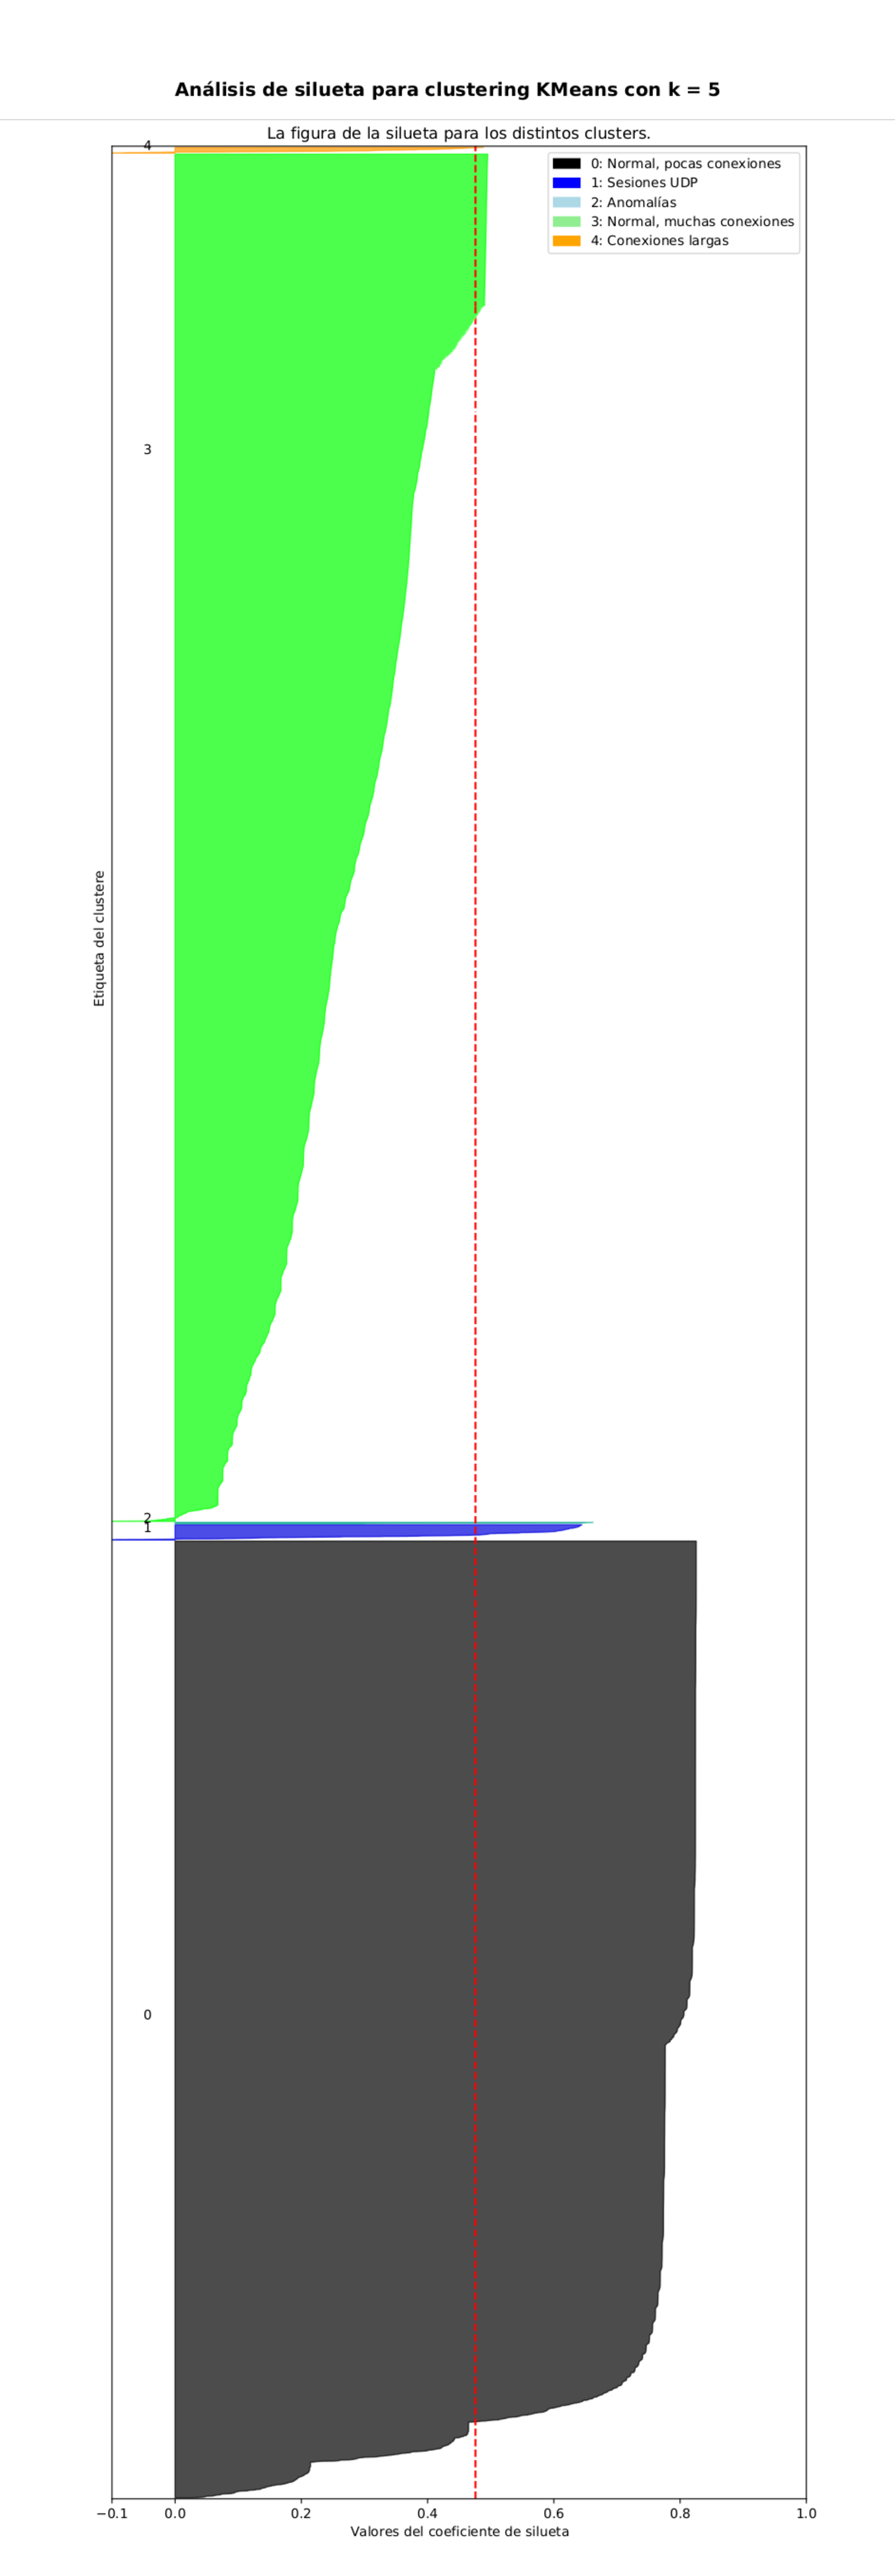
\includegraphics[height=\textheight]{contenido/fig/silhouette_cropped.pdf}
    \caption{Representación gráfica del análisis de silueta para los \emph{clusters} obtenidos con $k=5$}
    \label{fig:silhouette}
\end{figure}

\section{Valor de la contribución}\label{sec:valorcontribución}

[Valor de la contribución]

      \chapter{Conclusiones y líneas futuras}\label{chap:conclusiones}

Para acabar, en este capítulo se recoge el resumen final del problema tratado, cómo se ha abordado y qué respalda la validez de esta solución.
Esta síntesis se enfoca en informar del alcance y relevancia de la aportación.
Finalmente, se señalan las perspectivas de futuro que abre el trabajo desarrollado y cómo puede emplearse en el campo de la monitorización de redes empresariales.

\section{Conclusiones}\label{sec:conclusiones}

Se ha logrado modelar el comportamiento de los equipos informáticos en una red corporativa mediante métodos de \emph{clustering},
descubriendo de forma no supervisada varias clases de equipos que cursan tráfico normal,
y se han detectado de manera automática algunas IP origen anómalas por su cantidad de conexiones y eventos.
Esto amplía el alcance de la monitorización que se mantenía hasta ahora, con nuevas capacidades.

Se han contestado satisfactoriamente las tres cuestiones planteadas al inicio de esta investigación:
\begin{itemize}
    \item Si podemos clasificar las direcciones IP de una gran red empresarial en categorías relevantes según su comportamiento de red:

        Efectivamente las características extraídas de cada dirección IP han servido para categorizarlas.
    \item Cuáles serían esas categorías:

        Las categorías finales han sido 5:
        \begin{itemize}
            \item Comportamiento normal con muchas conexiones
            \item Comportamiento normal con pocas conexiones
            \item Sesiones UDP
            \item Conexiones largas / muchos puertos origen
            \item Anomalías: muchos eventos y conexiones
        \end{itemize}
    \item Si sereremos capaces de identificar comportamientos sospechosos en base a esta clasificación:

        Los equipos que han caído en la categoría de ``Anomalías'' ciertamente correspondían a comportamientos fuera de lo normal,
        lo cual ha servido para identificar actividades extrañas (aunque no necesariamente malintencionadas).
\end{itemize}

Por tanto, puede decirse que esta aportación tendrá una aplicación práctica inmediata.
A juzgar por el poco coste de computación y los satisfactorios indicadores de calidad medidos,
el conjunto de procesados diseñados para este sistema podrá integrarse en los sistemas actuales de monitorización,
programando su ejecución para que ofrezca las direcciones IP \emph{clusterizadas} cada día (especialmente el de las anomalías más destacadas) y un analista pueda revisarlas.

Mediante el contraste de información con otras fuentes, se ha podido confirmar que los comportamientos clasificados como anómalos
eran efectivamente casos excepcionales que se desvían de la actividad que presenta un equipo común en esta red.
Se espera que este cruce de información en la revisión por parte del analista, previo a la comunicación de la anomalía a los responsables de la administración de los equipos correspondientes,
incremente la fiabilidad de los casos comunicados y pueda evitar en la medida de lo posible falsos positivos.

Sin embargo, aunque los ensayos se han hecho sobre una cantidad suficiente de datos como para dar validez a las conclusiones extraídas,
cabría esperar que su funcionamiento en producción requiera de más pruebas en tiempo real y sobre periodos de datos más prolongados,
para perfeccionarlo y comprobar que los resultados alcanzan la calidad esperada.

A nivel personal, este trabajo ha servido para afianzar las nociones sobre aprendizaje automático no supervisado recibidas en este máster mediante su puesta en práctica sobre una aplicación real.
También se ha conseguido extender los conocimientos que se tenían sobre el \emph{clustering} y profundizar en la literatura académica alrededor de este tema,
con lo que se ha aprendido mucho sobre cómo se estudia y se aplica esta técnica en diversos campos, en especial en la clasificación de tráfico de red y la detección de anomalías.

\section{Líneas futuras}\label{sec:lineasfuturas}

En el entorno donde se ha desarrollado este proyecto se ha considerado oportuno dar continuidad a la investigación.
De momento se trata de un prototipo, pero con próximas iteraciones y experiencia añadida en el entorno real,
se puede refinar el concepto hasta lograr una herramienta de monitorización con un alto grado de utilidad y fiabilidad.

La ampliación de esta investigación podría dirigirse en los siguientes sentidos:
\begin{itemize}

\item Incluir otros firewalls como fuente de datos, que enriquezcan la base de la que se parte (además, quizás podrían correlarse y con ello resultar mucho más valiosos).

\item Trabajar sobre el seguimiento de los cambios de tendencia en los \emph{clusters} normales e incluso procesarlos con un segundo método de \emph{clustering}, que permita más granularidad a la hora de distinguir tipos de acciones habituales y descubra comportamientos particulares más sutiles.

\item Aplicar preprocesados y técnicas de \emph{clustering} similares a conexiones externas, para caracterizar el comportamiento de direcciones IP que se conecten a servicios públicos de la red de una empresa.

\item Enfocarse en el diseño de una forma de visualización adecuada para que el analista pueda comprender y revisar los resultados más fácilmente.

\end{itemize}

      \cleardoublepage
\phantomsection
\addcontentsline{toc}{chapter}{Bibliografía}
\printbibliography

      \begin{appendices}
        %Incluir aquí todos los apéndices (carpeta contenido).
        \chapter{Fusce viverra lectus}\label{app:one}


Nam viverra, odio et vulputate ultricies, sem libero ornare nunc, nec suscipit urna sapien eu sapien. Nulla erat nulla, hendrerit non elit vitae, venenatis malesuada libero. Duis ornare sapien sed lacus condimentum rutrum. Donec feugiat erat id elit aliquam, a ultrices lectus mattis. In vitae nisl tortor. Proin pellentesque nec odio et posuere. Ut aliquet quam ac magna tincidunt ultrices. Nullam sit amet elementum leo. Pellentesque vitae mi dolor. Pellentesque habitant morbi tristique senectus et netus et malesuada fames ac turpis egestas. Suspendisse tincidunt mi arcu, vitae porttitor mauris elementum ut.
      \end{appendices}
\end{document}
